\documentclass[12pt,letterpaper]{article}
\usepackage[utf8]{inputenc}
\usepackage{amsmath,amssymb,fullpage,graphicx}
\usepackage{subfigure}
\usepackage{amssymb}
\let\hat\widehat
\let\tilde\widetilde

\begin{document}
\subsection*{Q3-a}

\begin{verbatim}
baby_dt <- read.table("babiesI.data", sep = "", header=T)
baby_dt <- baby_dt[(baby_dt$smoke==0 | baby_dt$smoke==1),] 
# exclude unknown smoke status

hist(baby_dt[baby_dt$smoke==1,]$bwt, xlim=c(min(baby_dt$bwt),max(baby_dt$bwt)), 
     ylim=c(0, 0.027), breaks=30, probability = T, col=rgb(1,0,0,0.5),
     main='Distribution of Baby Weight', xlab='Baby Weight')
hist(baby_dt[baby_dt$smoke==0,]$bwt, probability = T, breaks=30, add=T, 
     col=rgb(0,0,1,0.5))
legend('topleft', c('Smoke', 'Non-Smoke'), 
       col=c(rgb(1,0,0,0.5),rgb(0,0,1,0.5)),lwd=3, cex = 0.7)
\end{verbatim}

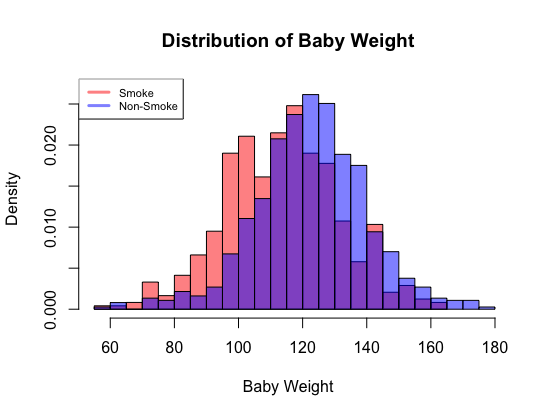
\includegraphics[width=150mm]{hist_babywt}

\begin{verbatim}
p <- ggplot(baby_dt, aes(status, bwt))
p + geom_boxplot(fill='skyblue') +
  labs(title="Boxplot of Baby Weight", 
       x="Smoke Status",
       y="Baby Weight") 
\end{verbatim}

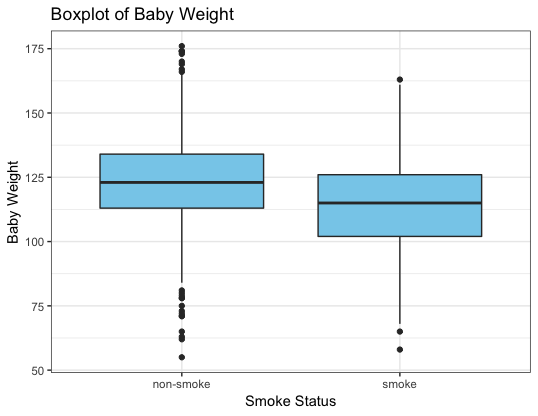
\includegraphics[width=150mm]{boxplot_babywt}

\begin{verbatim}
> summary(baby_dt[baby_dt$smoke==1,]$bwt)
   Min. 1st Qu.  Median    Mean 3rd Qu.    Max. 
   58.0   102.0   115.0   114.1   126.0   163.0 
> summary(baby_dt[baby_dt$smoke==0,]$bwt)
   Min. 1st Qu.  Median    Mean 3rd Qu.    Max. 
   55     113     123     123     134     176 
\end{verbatim}

\noindent The mean weight of baby whose mother smoked is 114.1, the median is 115, the standard deviation is 18.09895, and values range from 58 to 163 with interquartile 24. \\

\noindent Both the mean and median weight baby whose mother doesn't smoke are 123, the standard deviation is 17.39869, and values range from 55 to 176 with interquartile 21. \\

\noindent We may perceive from the histogram that distributions of baby weight of both smoker and non-smoker are approximately normal, but are slightly different on mean value (non-smokers' $>$ smokers'). \\

\noindent  The boxplot shows there are a outliers (1.5 times interquartiles above third quartile or below first quartile) on both groups. For smoke group, outliers are defined as values that exceed 162 or less than 66. For non-smoker group, outliers are thoes greater than 165.5 or less than 81.5. \\
\noindent Under this regulation there are 3 outliers in smoke group and 21 outliers in non-smoke group. 



\subsection*{Q3-b}
\noindent The distributions of two samples are approximately normal, so we may apply two sample t-test to check if the baby of smoked mother weighs less. \\

\noindent Let $W_1$ denotes the weight of a baby whose mother smoked, and $W_2$ denotes weight of whom mother doesn't smoke. \\

\noindent Let $\mu_1$ denotes true population mean of smoke mother's baby weight, and $\mu_2$ denotes true population mean of non-smoker mother's baby weight \\

\noindent $H_0$: $\mu_1 = \mu_2$ \\
\noindent $H_1$: $\mu_1 < \mu_2$ \\

\noindent The t-statistic is defined as 

\begin{align*}
T &= \frac{\bar{W_1}- \bar{W_2}}{\sqrt[]{\frac{S_{W_1}^2}{n_1} + \frac{S_{W_2}^2}{n_2}}} \text{ with df} = n_1 + n_2 - 2
\end{align*}


\noindent We have calculated $\bar{W_1} = 114.1$, $\bar{W_2} = 123$, $sd(W_1) = 18.1$, $sd(W_2) = 17.4$, and the sample size $n_1 = 484$, $n_2 = 742$ as well. 

\begin{align*}
T &= \frac{114.1 - 123}{\sqrt[]{\frac{18.1^2}{484} + \frac{17.4^2}{742}}} \\
&\approx  -8.58 \text{, df = 1224}
\end{align*}

\begin{verbatim}
> pt(-8.58, df=1224)
[1] 1.415762e-17
\end{verbatim}

\noindent P-value is $1.42 \times 10^{-17} < 0.01$\\

\noindent P-value calculated from R t.test turns out to be $2.2 \times 10^{-16}$ due to difference in calculated degree of freedom (in t.test, the calculated df is 1003). In both way, p-value is extremely small. \\

\noindent Therefore, under the test size $\alpha = 0.01$, we may reject the null which states mean baby weight of two groups are the same. But we may not directly accept the alternative statement, due to unknown power of the test.


\end{document}